\documentclass[t, notes, xcolor=table]{beamer}

\usepackage{wrapfig}
\usepackage{float}
% For tabs in verbatim
\usepackage{fancyvrb}

% Adjust position of the image
\usepackage[export]{adjustbox}

% set fonts
\usefonttheme{professionalfonts} % using non standard fonts for beamer
\usepackage{txfonts,mathptmx}

% set indend spacing for first and second level indentation
\setlength{\leftmargini}{0.5cm}
\setlength{\leftmarginii}{0.5cm}
\setlength{\leftmarginiii}{0.5cm}

% Set circles for bullets 
\setbeamertemplate{itemize items}[circle]

% colors
\usepackage{xcolor}

% multiple columns
\usepackage{multicol}

% todo lists
\usepackage{pifont}
\usepackage{amssymb}

% increase space between text and frame name
\addtobeamertemplate{frametitle}{}{\vspace{0.5em}}

%Information to be included in the title page:
\title{Designing Finite State Machines}
\author{Nikola Petrovic}
\institute{University of Belgrade, School of Electrical Engineering}
\date{2022}



\begin{document}

\frame{\titlepage}

%%%%%%%%%%%%%%%%%%%%%%%%%%%%%%%%%%%%%%%%%%%%%%%%%%%%%%%%%%%%
\begin{frame}
\frametitle{Module Objective}
In this module we will code state machines for synthesis.
\newline

\textbf{Topics:}
\begin{itemize}
\item FSM introduction
\item Defining the FSM states
\item Example read-write synchronizer FSM
\item Coding FSMs in various styles
\item Various ways to optimize FSMs
\end{itemize}
\end{frame}
\note{
\scriptsize{
Your objective is to code state machines for synthesis.
\newline

To help you do that, this module discusses what an FSM is, how to define FSM states, various ways to code FSMs for synthesis, and various ways to optimize FSMs.

}
}

%%%%%%%%%%%%%%%%%%%%%%%%%%%%%%%%%%%%%%%%%%%%%%%%%%%%%%%%%%%%
\begin{frame}
\frametitle{Finite State Machine (FSM) Review}
\scriptsize{
\begin{multicols}{2}
\textbf{FSM Structure}
\begin{itemize}
\item State Register
\begin{itemize}
	\scriptsize{
	\item[$-$] Stores current state
	}
\end{itemize}
\item Next State decode logic
\begin{itemize}
	\scriptsize{
	\item[$-$] Decides next state based on current state and
inputs
	}
\end{itemize}
\item Output Logic
\begin{itemize}
	\scriptsize{
	\item[$-$] Decodes state (or states and inputs) to produce
	}
outputs
\end{itemize}
\item Outputs from the FSM can be a function of:
\begin{itemize}
	\scriptsize{
	\item[$-$] Current state only – \textbf{Moore}
	\item[$-$] Current state and the current inputs – \textbf{Mealy}
	}
\end{itemize}
\end{itemize}
\vfill
\columnbreak
\begin{figure}
    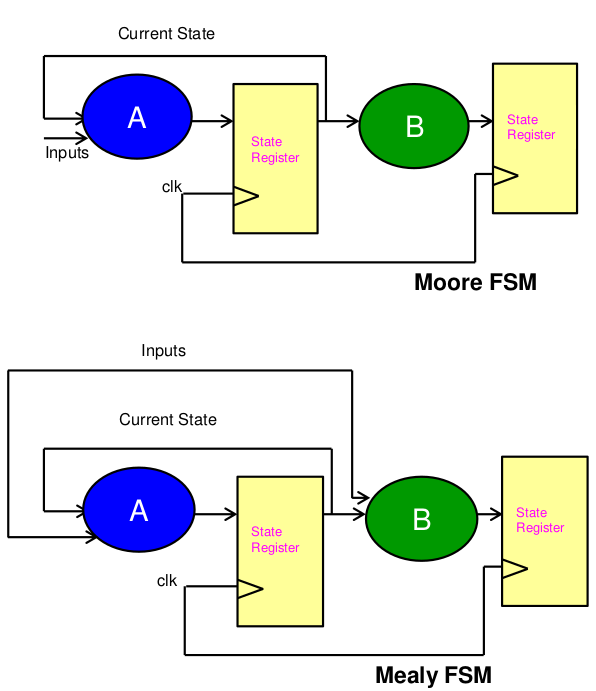
\includegraphics[width=0.45\textwidth]{img/14_FSM_review.png}
\end{figure}
\end{multicols}
}
\end{frame}
\note{
\scriptsize{
An FSM consists of state-encoding combinational logic, state-storing sequential elements, and output-decoding combinational logic.
\begin{itemize}
\item A Moore machine has no combinational path from inputs to outputs. The outputs are a function solely of the current state vector.
\item A Mealy machine has at least one combinational from an input to an output. The outputs are a function of the current state and at least one current input. Mealy outputs can be available up to one clock earlier path than Moore outputs, but may complicate synthesis timing constraint definition.
\end{itemize}

If the current state of your design depends at least partially upon the previous state, then your design is
an FSM.
\newline

--------

Perhaps one way to remember which is the Mealy machine and which is the Moore machine is the phrase "Mealy is more and Moore is less". This refers to the outputs, which in the Mealy machine can include unregistered inputs.

}
}

%%%%%%%%%%%%%%%%%%%%%%%%%%%%%%%%%%%%%%%%%%%%%%%%%%%%%%%%%%%%
\begin{frame}
\frametitle{Defining the FSM States}
\scriptsize{
\begin{itemize}
\item You will likely see FSM descriptions that define state vector values with text replacement macros.
\item This training does not do that and you should neither.
\end{itemize}

\begin{figure}
    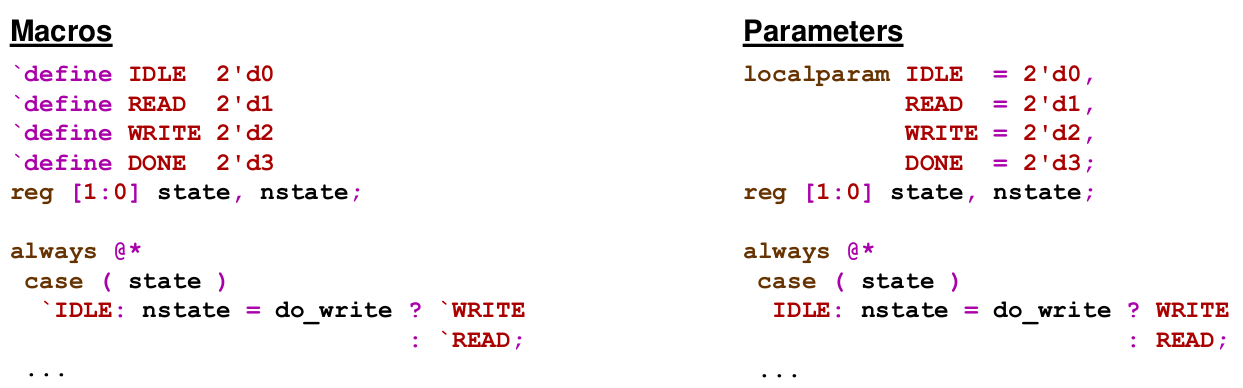
\includegraphics[width=0.95\textwidth]{img/14_FSM_def.png}
\end{figure}
\begin{multicols}{2}
\begin{itemize}
\item Scope is global – across files and modules from `define to `undef
\item Accepted by synthesis tools but not for FSM optimization
\end{itemize}
\vfill
\columnbreak
\begin{itemize}
\item Scope is local to declaring block
\item Required by synthesis tools that perform FSM optimizations
\end{itemize}
\end{multicols}
}
\end{frame}
\note{
\scriptsize{
The scope of any compiler directive is from the point of the direction to the point of its redirection or removal, potentially across multiple files and multiple modules. To inadvertently use a macro defined elsewhere or to define a macro inadvertently used elsewhere is very easy. To help prevent such erroneous use, designers typically place text macro definitions in a separate file that any compilation unit that uses the definitions includes during compilation. This encapsulates those definitions in a single easily-modified place.
\newline

The scope of a local parameter is the declaring block. No code can change its initialized value.
\newline

Synthesis tools that perform state machine optimizations require you to define the states with parameters if you want the tool to perform the optimizations.

}
}

%%%%%%%%%%%%%%%%%%%%%%%%%%%%%%%%%%%%%%%%%%%%%%%%%%%%%%%%%%%%
\begin{frame}
\frametitle{Example Read-Write Synchronizer FSM}
\footnotesize{
The following examples refer to this FSM specification:
\begin{itemize}

\item If do\_write is true, transition to WRITE and set exec = 0 and rd\_wr = 1.
\begin{itemize}
\scriptsize{
	\item[$-$] When do\_write is again true, transition to DONE and set exec = 1.
}
\end{itemize}
\item If do\_write is false, transition to READ and set exec = 0 and rd\_wr = 0.
\begin{itemize}
\scriptsize{
	\item[$-$] When do\_write is again false, transition to DONE and set exec = 1.
}
\end{itemize}

\end{itemize}
\begin{figure}
    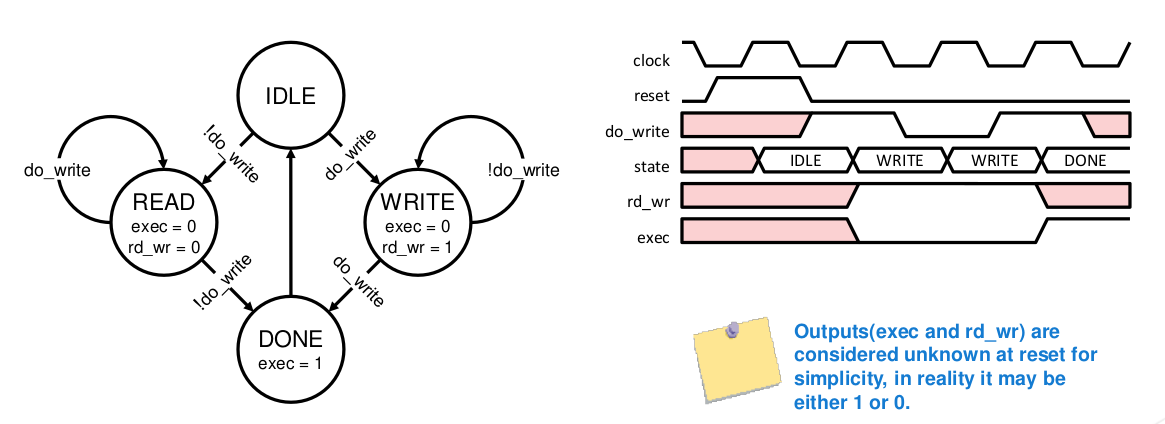
\includegraphics[width=0.95\textwidth]{img/14_FSM_ex.png}
\end{figure}
}
\end{frame}
\note{
\scriptsize{
The following examples refer to this FSM specification:
\begin{itemize}

\item If do\_write is true, transition to WRITE and set exec = 0 and rd\_wr = 1.
\begin{itemize}
\scriptsize{
	\item[$-$] When do\_write is again true, transition to DONE and set exec = 1.
}
\end{itemize}
\item If do\_write is false, transition to READ and set exec = 0 and rd\_wr = 0.
\begin{itemize}
\scriptsize{
	\item[$-$] When do\_write is again false, transition to DONE and set exec = 1.
}
\end{itemize}
\end{itemize}
}
}

%%%%%%%%%%%%%%%%%%%%%%%%%%%%%%%%%%%%%%%%%%%%%%%%%%%%%%%%%%%%
\begin{frame}
\frametitle{Coding the FSM in One Block: Sequential Outputs}
\begin{figure}
    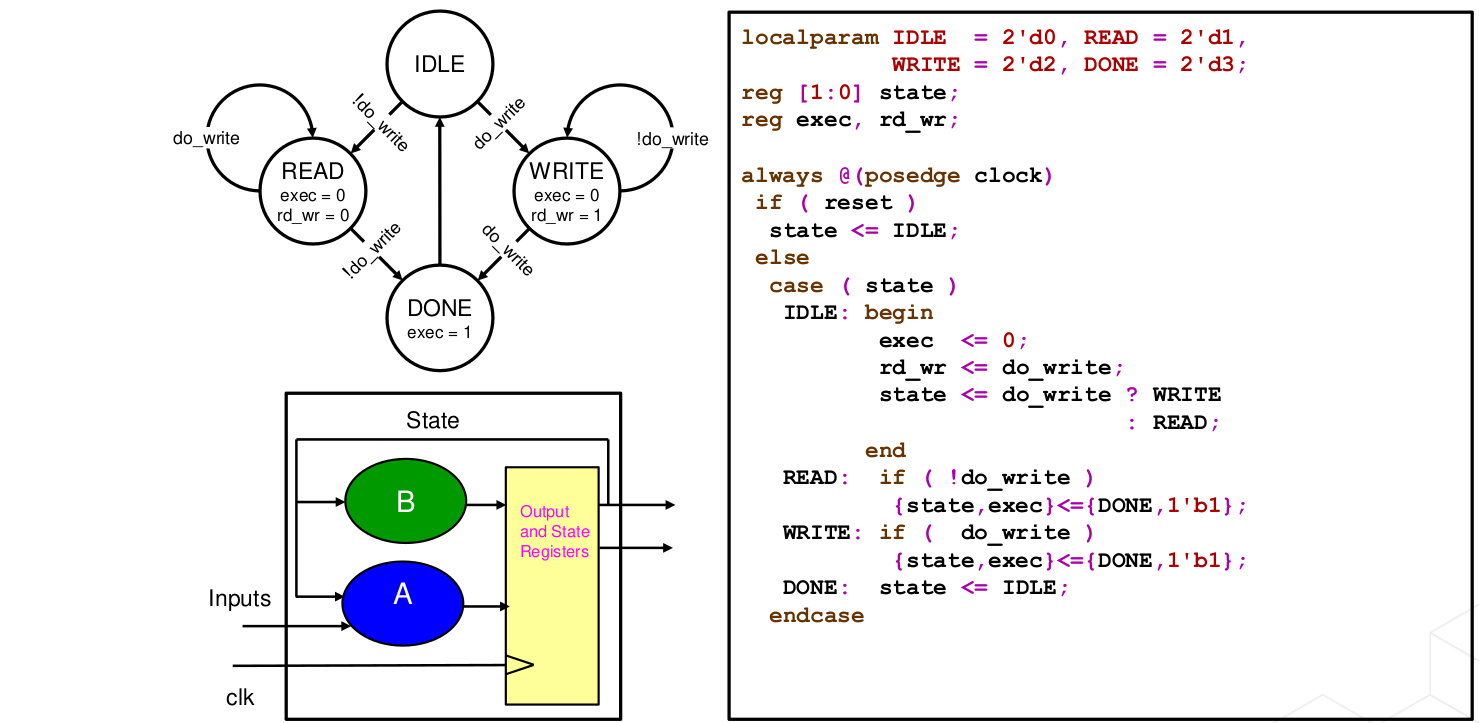
\includegraphics[width=0.95\textwidth]{img/14_FSM_coding.png}
\end{figure}
\end{frame}
\note{
\scriptsize{
The one-block coding style generates the next-state, state, and outputs all in one sequential block.
}
}

%%%%%%%%%%%%%%%%%%%%%%%%%%%%%%%%%%%%%%%%%%%%%%%%%%%%%%%%%%%%
\begin{frame}
\frametitle{Coding the FSM in Two Blocks: Sequential Outputs}
\begin{figure}
    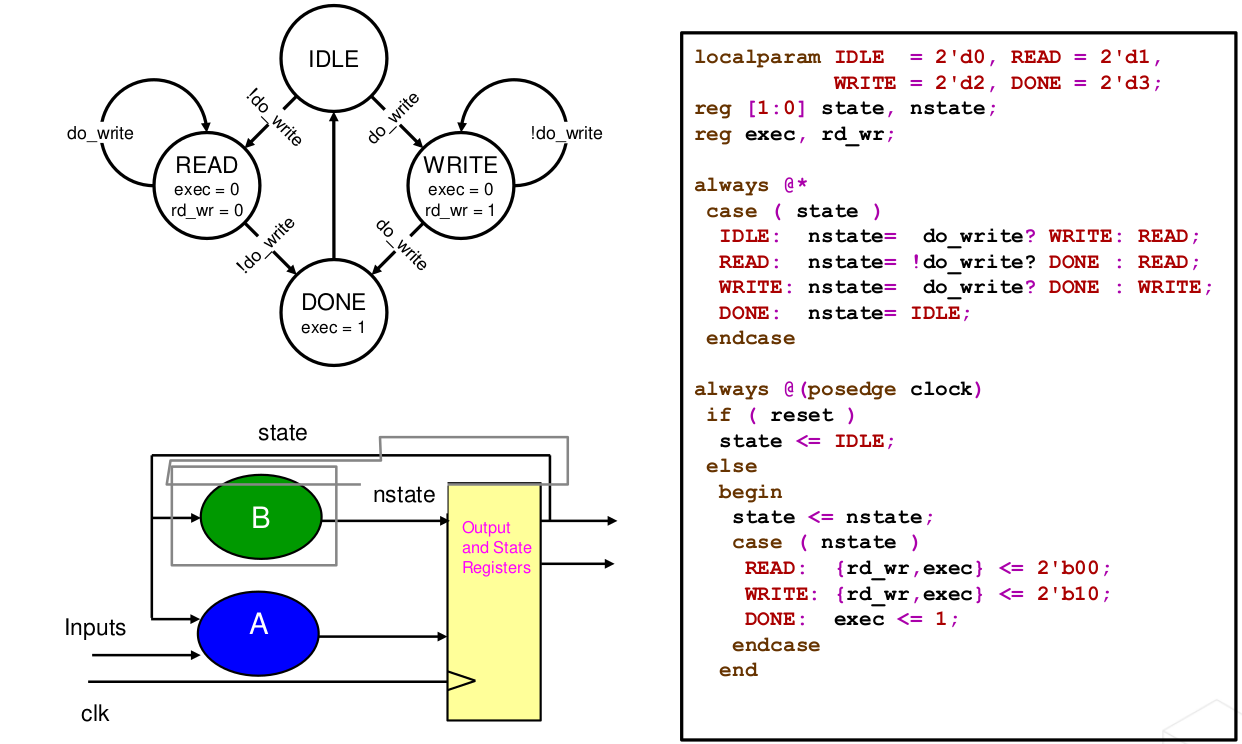
\includegraphics[width=0.95\textwidth]{img/14_FSM_coding_two.png}
\end{figure}
\end{frame}
\note{
\scriptsize{
The two-block coding style encodes the next state in a separate combinational block. You must place asynchronous reset in the sequential block. You can place synchronous reset in either block, but synthesis tools might more accurately identify the components reset pin if you place the reset in the sequential block.

}
}

%%%%%%%%%%%%%%%%%%%%%%%%%%%%%%%%%%%%%%%%%%%%%%%%%%%%%%%%%%%%
\begin{frame}
\frametitle{Coding the FSM in Three Blocks: Sequential Outputs}
\begin{figure}
    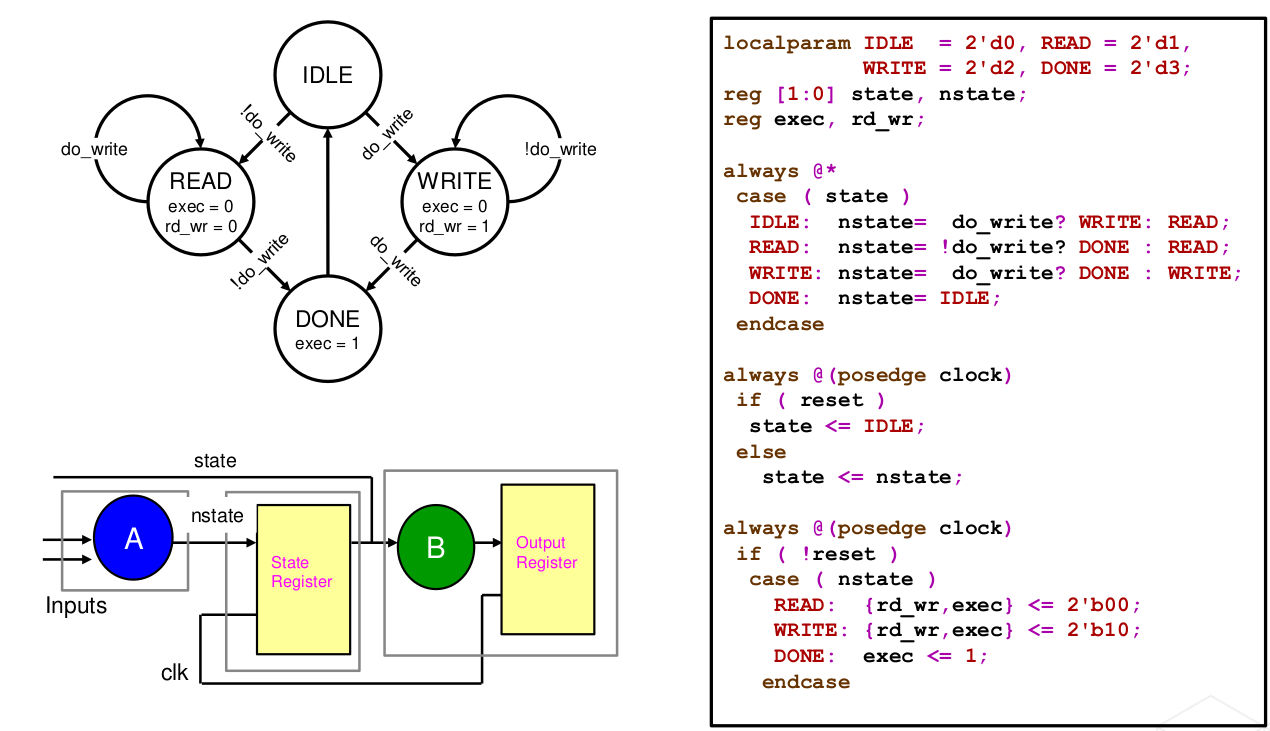
\includegraphics[width=0.95\textwidth]{img/14_FSM_coding_three.png}
\end{figure}
\end{frame}
\note{
\scriptsize{
The three-block coding style decodes the outputs in a third block. Here, that third block is sequential.
\newline

Note that the outputs do not transition while the reset is active.

}
}

%%%%%%%%%%%%%%%%%%%%%%%%%%%%%%%%%%%%%%%%%%%%%%%%%%%%%%%%%%%%
\begin{frame}
\frametitle{Coding in Three Blocks: Combinational Outputs}
\begin{figure}
    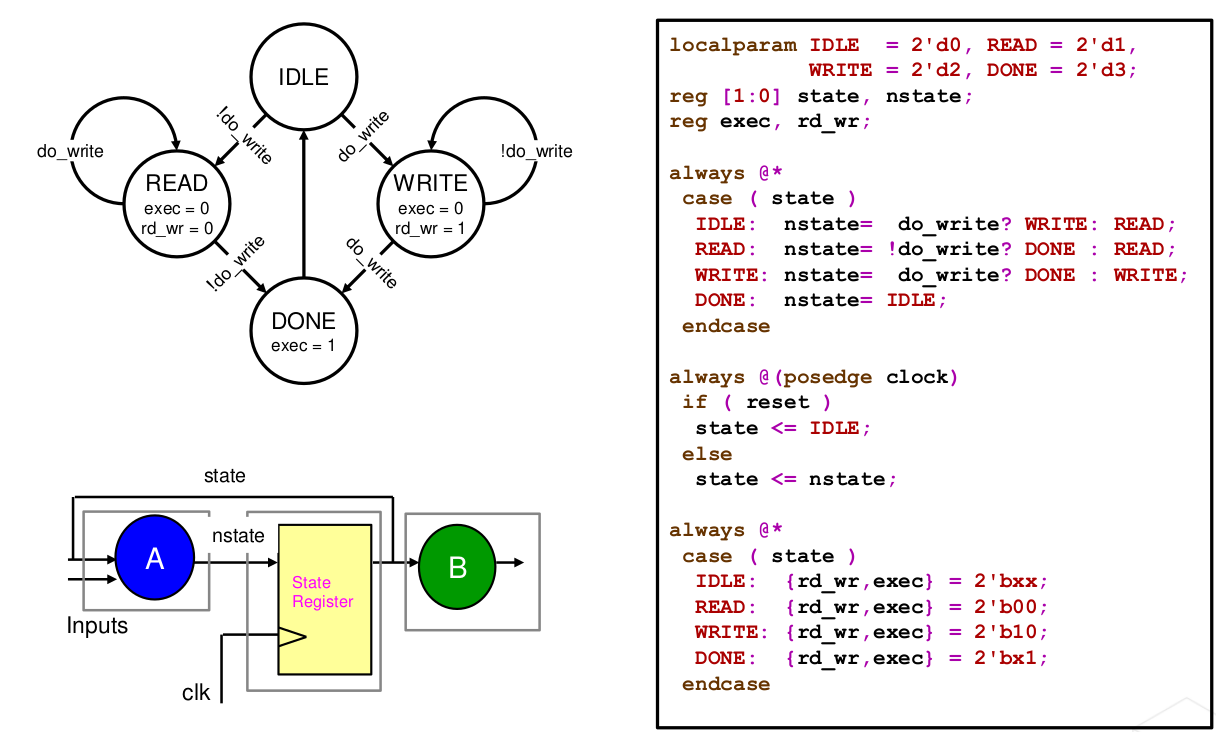
\includegraphics[width=0.95\textwidth]{img/14_FSM_coding_three_comb.png}
\end{figure}
\end{frame}
\note{
\scriptsize{
The three-block coding style decodes the outputs in a third block. Here, that third block is combinational. The combinational block takes advantage of the specification that for some states we do not care what the output value is.

}
}

%%%%%%%%%%%%%%%%%%%%%%%%%%%%%%%%%%%%%%%%%%%%%%%%%%%%%%%%%%%%
\begin{frame}
\frametitle{Optimizing Register Count}

\scriptsize{
\begin{multicols}{2}
\begin{itemize}
\item Registering outputs is preferable for synthesis as it
simplifies timing constraints.
\item Examine the mapping between state and output.
\item Can output registers replace state bits? If so then you can reduce your overall register count.
\end{itemize}
\vfill
\begin{figure}
    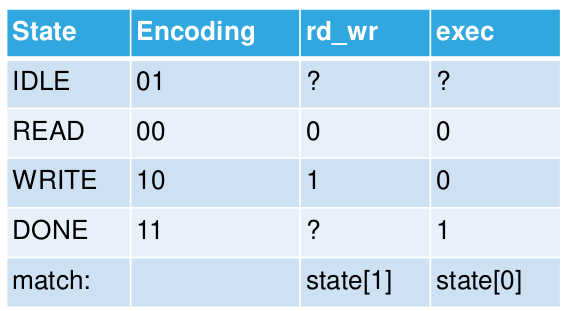
\includegraphics[width=0.45\textwidth]{img/14_FSM_optimize.png}
\end{figure}
\columnbreak
\begin{figure}
    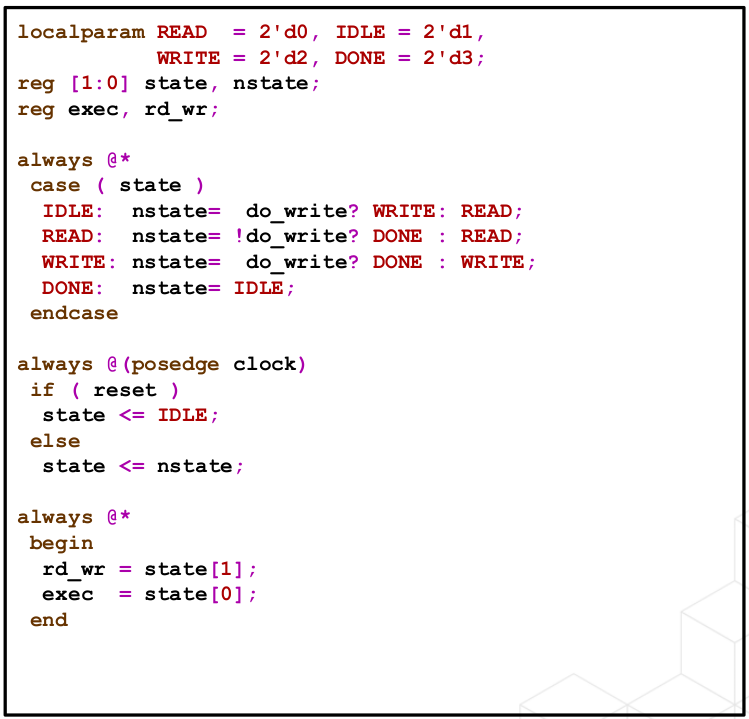
\includegraphics[width=0.55\textwidth]{img/14_FSM_optimize2.png}
\end{figure}
\end{multicols}
}
\end{frame}


%%%%%%%%%%%%%%%%%%%%%%%%%%%%%%%%%%%%%%%%%%%%%%%%%%%%%%%%%%%%
\begin{frame}
\frametitle{Module}

\end{frame}
\note{
\scriptsize{

}
}

%%%%%%%%%%%%%%%%%%%%%%%%%%%%%%%%%%%%%%%%%%%%%%%%%%%%%%%%%%%%
\begin{frame}
\frametitle{Optimizing Power and Noise: Gray Encoding}
\scriptsize{
Where vectors regularly traverse a range of values, opportunities exist to encode values in consideration of power efficiency and noise reduction. Perhaps the most classic of examples is Gray-encoded counting.
}
\vfill
\begin{figure}
    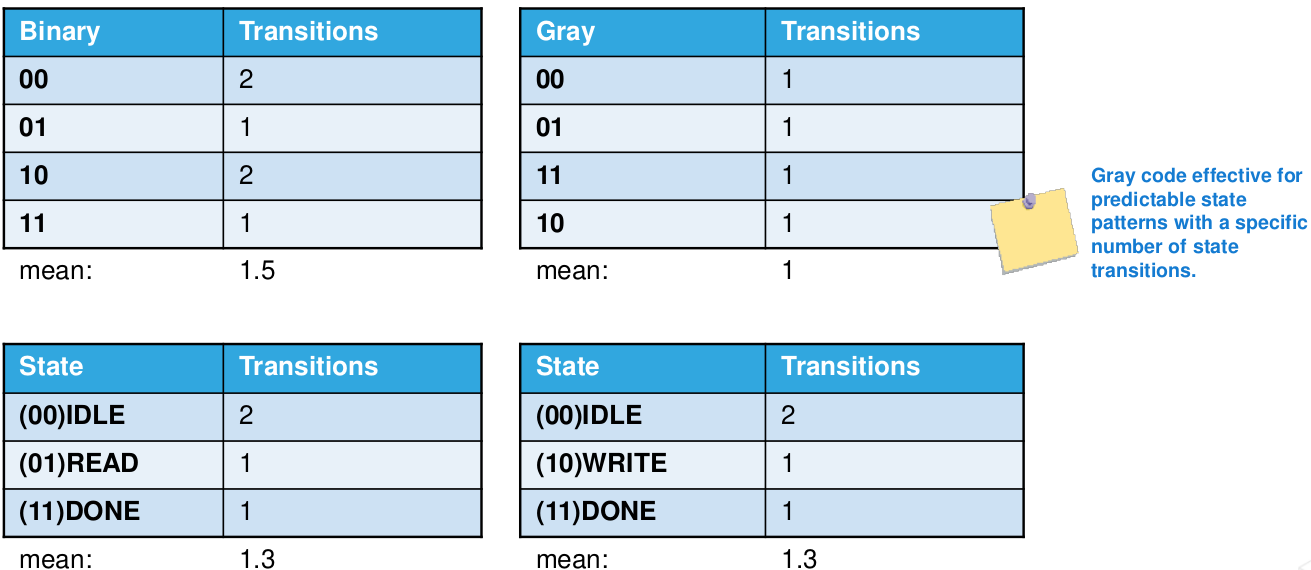
\includegraphics[width=0.95\textwidth]{img/14_FSM_optimize_power.png}
\end{figure}
\end{frame}
\note{
\scriptsize{
Bell Labs researcher Frank Gray applied for patent 2,632,058 "Pulse Code Communication" in 1947, defining a "reflected binary code" for lack of a better term. Coincidentally with the patent award, the codes became popularly known as Gray codes. A Gray code is "a binary numeral system where two successive values differ in only one digit" – http://en.wikipedia.org/wiki/Gray\_code
\newline

The tabulated sequence is the original "binary reflected Gray code" (that you can generate from binary using $g=b\wedge(b>>1)$)but other Gray codes also exist.
\newline

While initially used to work around switch-bounce, as the new vector value can be used immediately without further waiting for the value to "settle", gray-encoding is indispensable for address counters that increment in one clock domain and are read in another, for example in asynchronous FIFOs.
\newline

Gray-encoding has more recently become valuable in the quest for reduced switching activity. The simple counting sequence displayed here averages 1.5 transitions per clock for binary encoding and 1 transition per clock for Gray encoding.
\newline

Paths through the example machine have a length of only three states, so present little opportunity to reduce switching activity.

}
}

%%%%%%%%%%%%%%%%%%%%%%%%%%%%%%%%%%%%%%%%%%%%%%%%%%%%%%%%%%%%
\begin{frame}
\frametitle{Optimizing Performance: One-Hot Encoding}

\begin{figure}[t]
    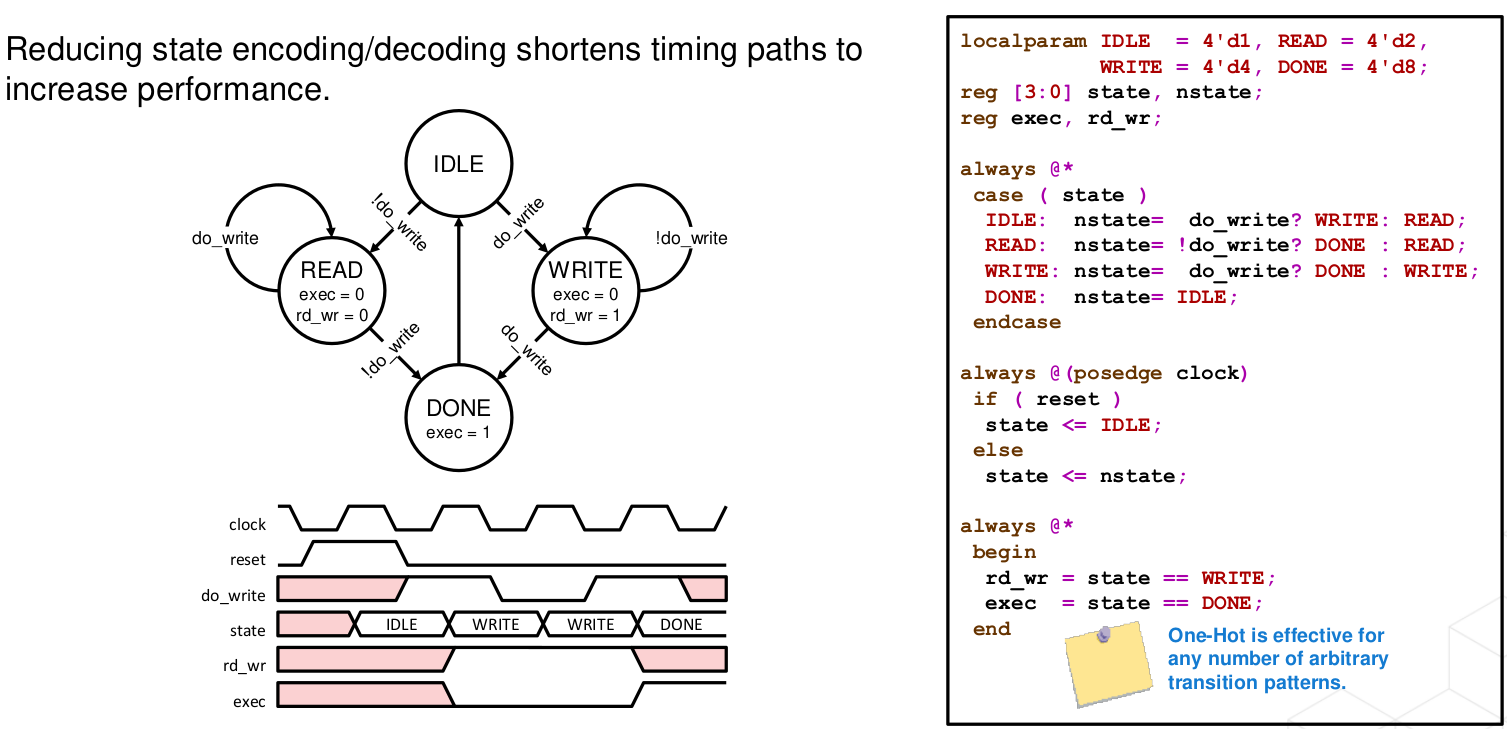
\includegraphics[width=1\textwidth]{img/14_FSM_optimize_perf.png}
\end{figure}

\vfill
\end{frame}
\note{
\scriptsize{
One-hot state encoding provides a unique state bit for each state. This reduces the combinational logic required to encode and decode the state, thus shortens the timing path to permit increased clock speed.

}
}

%%%%%%%%%%%%%%%%%%%%%%%%%%%%%%%%%%%%%%%%%%%%%%%%%%%%%%%%%%%%
\begin{frame}
\frametitle{One-Hot Encoding by Indexing State Bits}
\begin{figure}[t]
    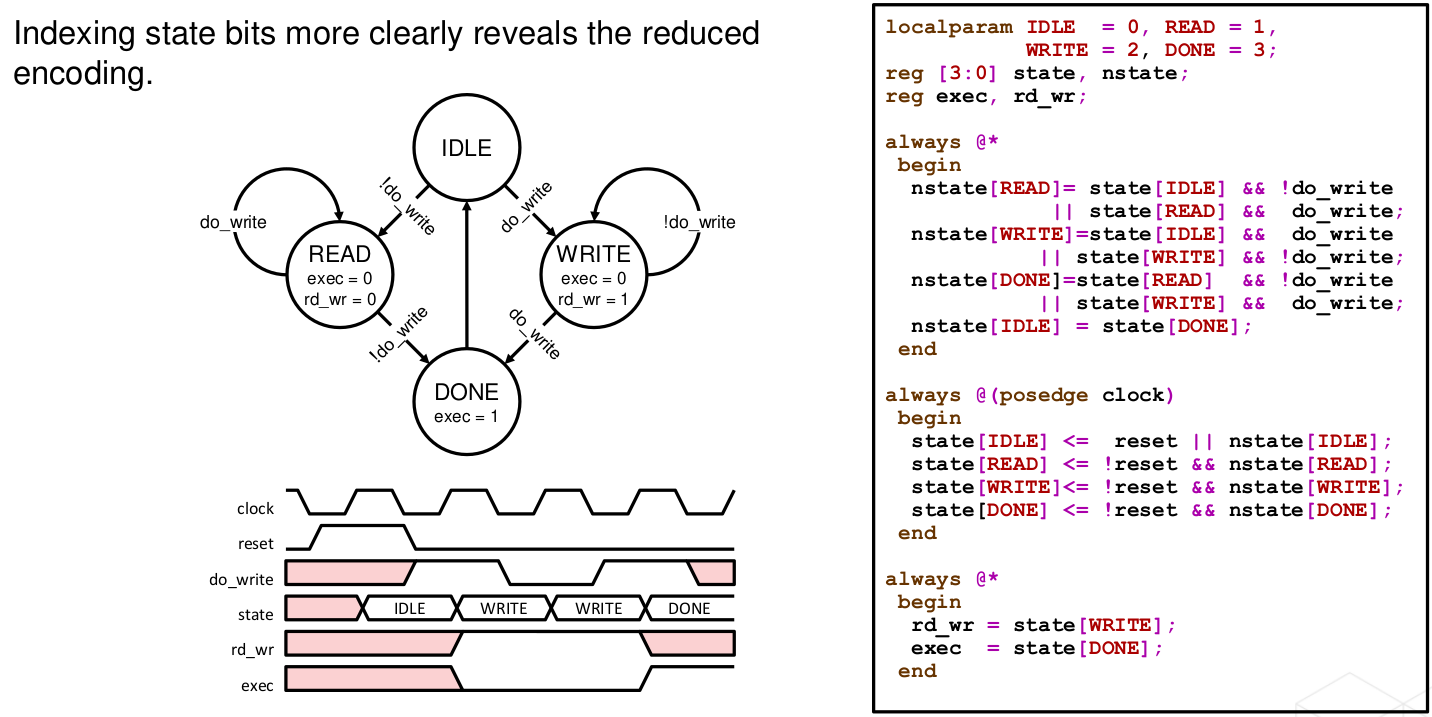
\includegraphics[width=1\textwidth]{img/14_FSM_optimize_one_hot.png}
\end{figure}
\end{frame}
\note{
\scriptsize{
You can code the one-hot machine in a style that individually references each state bit. This style may more clearly reveal the reduced state encoding. Here, the longest path to any state bit is a sum of two products of three terms each.

}
}

%%%%%%%%%%%%%%%%%%%%%%%%%%%%%%%%%%%%%%%%%%%%%%%%%%%%%%%%%%%%
\begin{frame}
\frametitle{Module Summary}
We should now be able to code state machines for synthesis.
\newline

This module discussed:
\begin{itemize}
\item What is a FSM
\begin{itemize}
	\item State encoding, storage, and decoding
\end{itemize}
\item How to define FSM states
\begin{itemize}
	\item By use of local constants
\end{itemize}
\item Various ways to code FSMs for synthesis
\begin{itemize}
	\item 1-block, 2-block, 3-block
\end{itemize}
\item Various ways to optimize FSMs
\begin{itemize}
	\item For area, power, noise, performance
\end{itemize}
\end{itemize}
\end{frame}
\note{
\scriptsize{
You should now be able to code state machines for synthesis.
\newline

This module discussed what an FSM is, how to define FSM states, various ways to code FSMs for synthesis, and various ways to optimize FSMs.

}
}

%%%%%%%%%%%%%%%%%%%%%%%%%%%%%%%%%%%%%%%%%%%%%%%%%%%%%%%%%%%%
\begin{frame}
\frametitle{Module Review}
\begin{enumerate}
\item What is the difference between a Moore machine and a Mealy machine?
\item Why should you define state values using parameters instead of macros?
\item In how many blocks should you define the FSM to generate the best quality netlist?
\end{enumerate}
\end{frame}
\note{
\scriptsize{
\begin{enumerate}
\item What is the difference between a Moore machine and a Mealy machine?
\begin{itemize}
\scriptsize{
	\item The outputs of a Moore machine are a function purely of the machine state. The outputs of a Mealy machine are a function partially of at least one machine input.
}
\end{itemize}
\item Why should you define state values using parameters instead of macros?
\begin{itemize}
\scriptsize{
	\item A synthesis tool is more likely to recognize a state machine if you define state values using parameters instead of macros. Recognizing the state machine permits optimizations such as Gray or one-hot encoding.
}
\end{itemize}
\item In how many blocks should you define the FSM to generate the best quality netlist?
\begin{itemize}
\scriptsize{
	\item The netlist quality does not generally depend upon the number of blocks. Choose a number that clearly communicates your design intention.
}
\end{itemize}
\end{enumerate}

}
}

%%%%%%%%%%%%%%%%%%%%%%%%%%%%%%%%%%%%%%%%%%%%%%%%%%%%%%%%%%%%
\begin{frame}
\frametitle{Module Exercise}
\scriptsize{
Architect and code a FSM that outputs a "one" for one clock whenever it recognizes two adjacent ones in the input stream.
}
\begin{figure}
    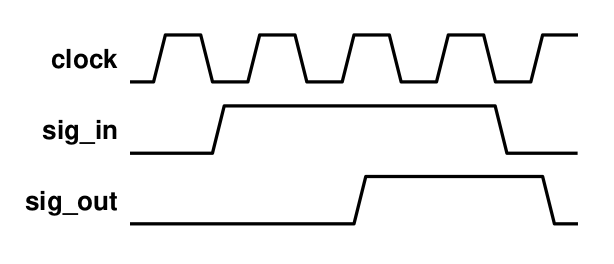
\includegraphics[width=0.45\textwidth]{img/14_ex.png}
\end{figure}
\end{frame}
\note{
\scriptsize{
\begin{figure}
    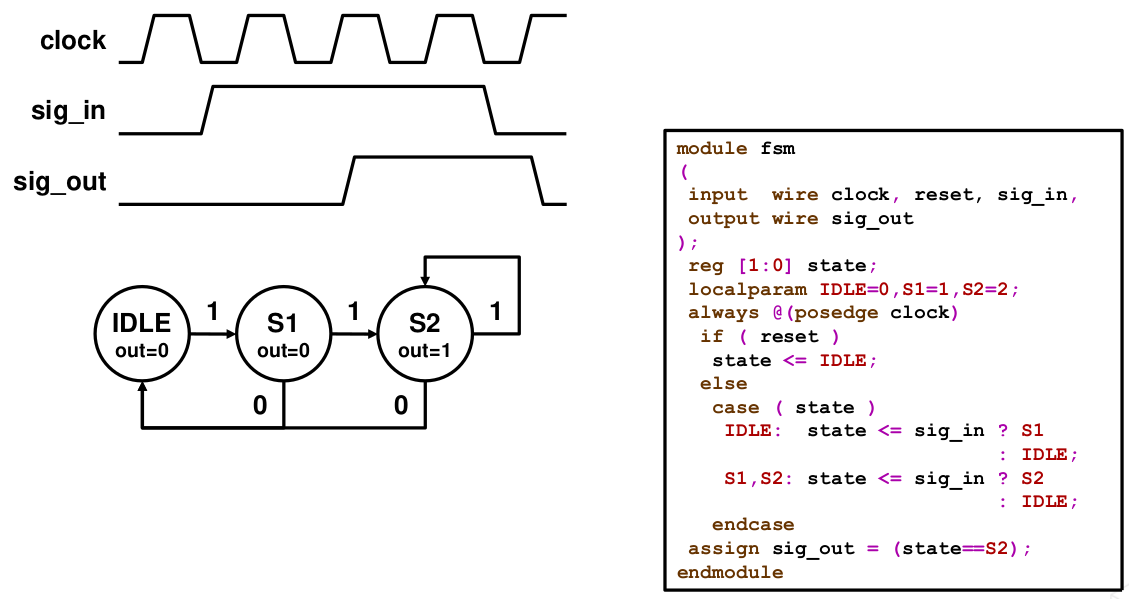
\includegraphics[width=0.95\textwidth]{img/14_ex_sol.png}
\end{figure}
}
}

%%%%%%%%%%%%%%%%%%%%%%%%%%%%%%%%%%%%%%%%%%%%%%%%%%%%%%%%%%%%
\begin{frame}
\frametitle{Lab}
Lab 14-1: Coding State Machines in Multiple Styles
\scriptsize{
\begin{itemize}
\item Code state machines in various styles for synthesis.
\item For this lab, you code the serial-to-parallel interface receiver as an FSM in different styles.
\end{itemize}
}
\end{frame}
\note{
\scriptsize{
Your objective for this lab is to code state machines for synthesis.
\newline

For this lab, you practice recoding a provided FSM to the styles that this module presented.

}
}


%%%%%%%%%%%%%%%%%%%%%%%%%%%%%%%%%%%%%%%%%%%%%%%%%%%%%%%%%%%%
\begin{frame}
\frametitle{Test You Understanding - 1}
For your FSM all output timing path originate at the clock. This is which FSM machine?
\begin{itemize}
\item[$\square$] mealy
\item[$\square$] moore
\end{itemize}
\end{frame}
\note{
\scriptsize{
For your FSM all output timing path originate at the clock. This is which FSM machine?
\begin{itemize}
\item[$\square$] mealy
\item[$\boxtimes$] moore
\end{itemize}
}
}

%%%%%%%%%%%%%%%%%%%%%%%%%%%%%%%%%%%%%%%%%%%%%%%%%%%%%%%%%%%%
\begin{frame}
\frametitle{Test You Understanding - 2}
You define FSM states with constants instead of text macros primarily because:
\begin{itemize}
\item[$\square$] synthesis tool can then do FSM optimization
\item[$\square$] all constants are visible across the entire design
\item[$\square$] synthesis tool do not except text macros
\end{itemize}
\end{frame}
\note{
\scriptsize{
You define FSM states with constants instead of text macros primarily because:
\begin{itemize}
\item[$\boxtimes$] synthesis tool can then do FSM optimization
\item[$\square$] all constants are visible across the entire design
\item[$\square$] synthesis tool do not except text macros
\end{itemize}
}
}

%%%%%%%%%%%%%%%%%%%%%%%%%%%%%%%%%%%%%%%%%%%%%%%%%%%%%%%%%%%%
\begin{frame}
\frametitle{Test You Understanding - 3}
In how many blocks should you define the FSM to generate the best quality netlist?
\begin{itemize}
\item[$\square$] 1
\item[$\square$] 2
\item[$\square$] 3
\item[$\square$] any number
\end{itemize}
\end{frame}
\note{
\scriptsize{
In how many blocks should you define the FSM to generate the best quality netlist?
\begin{itemize}
\item[$\square$] 1
\item[$\square$] 2
\item[$\square$] 3
\item[$\boxtimes$] any number
\end{itemize}
}
}

%%%%%%%%%%%%%%%%%%%%%%%%%%%%%%%%%%%%%%%%%%%%%%%%%%%%%%%%%%%%
\begin{frame}
\frametitle{Test You Understanding - 4}
You would use Gray state encoding primarily to optimize:
\begin{itemize}
\item[$\square$] congestion
\item[$\square$] power
\item[$\square$] speed
\item[$\square$] area
\end{itemize}
\end{frame}
\note{
\scriptsize{
You would use Gray state encoding primarily to optimize:
\begin{itemize}
\item[$\square$] congestion
\item[$\boxtimes$] power
\item[$\square$] speed
\item[$\square$] area
\end{itemize}
}
}



\end{document}
